\cabecalho

\section*{Exercícios}

\begin{enumerate}

    \item Verificar $FLA$, $FLM$, $FLT$ para a viga birrotulada VSM 450 x 68, aço USICIVIL 350.
    
    \input{assets/images/viga2.tex}

    \begin{tikzpicture}[>=stealth]
    % Eixo X (Vermelho)
    \draw [->, thick, black] (0,0,0) -- (2,0,0) node [right] {$z$};
    
    % Eixo Y (Verde)
    \draw [->, thick, black] (0,0,0) -- (0,2,0) node [above] {$y$};
    
    % Eixo Z (Azul)
    \draw [->, thick, black] (0,0,0) -- (0,0,2) node [below left] {$x$};
\end{tikzpicture}

    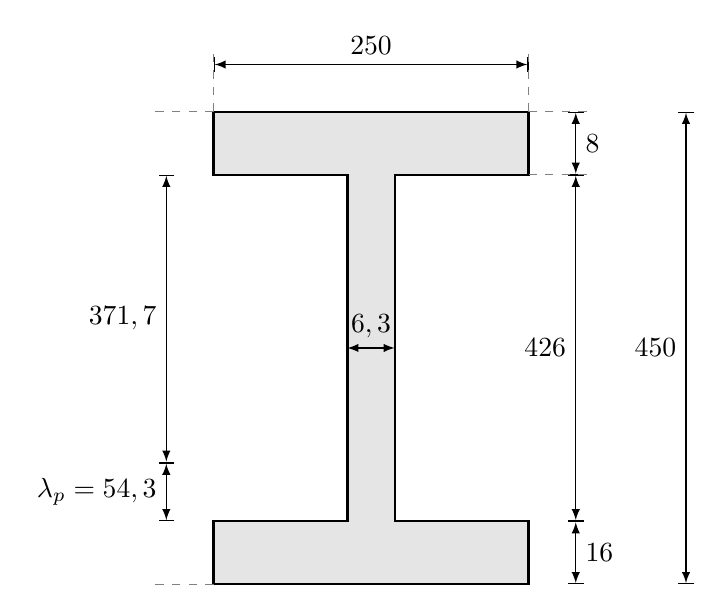
\begin{tikzpicture}[
    % Configuração global das setas de cota para ficarem com aparência técnica
    cota/.style={|<->|, >=latex, thin},
    % Estilo da linha do perfil
    perfil/.style={thick, fill=gray!20, draw=black}
]

    % ==========================================
    % 1. DESENHANDO O PERFIL I (Coordenadas)
    % ==========================================
    % Consideraremos as seguintes medidas base para o desenho:
    % Largura da mesa (bf) = 4cm (de x=-2 até x=2)
    % Altura total (d) = 6cm (de y=0 até y=6)
    % Espessura da mesa (tf) = 0.8cm
    % Espessura da alma (tw) = 0.6cm (de x=-0.3 a x=0.3)
    
    \draw[perfil] 
        (-2, 0) -- (2, 0)          % Base inferior
        -- (2, 0.8)                % Sobe a lateral direita da mesa inferior
        -- (0.3, 0.8)              % Entra em direção à alma
        -- (0.3, 5.2)              % Sobe a alma pelo lado direito
        -- (2, 5.2)                % Sai para a direita na mesa superior
        -- (2, 6)                  % Sobe a lateral direita da mesa superior
        -- (-2, 6)                 % Topo superior
        -- (-2, 5.2)               % Desce a lateral esquerda da mesa superior
        -- (-0.3, 5.2)             % Entra em direção à alma
        -- (-0.3, 0.8)             % Desce a alma pelo lado esquerdo
        -- (-2, 0.8)               % Sai para a esquerda na mesa inferior
        -- cycle;                  % Fecha o caminho de volta ao (-2,0)


    % ==========================================
    % 2. DESENHANDO AS COTAS (Linhas de dimensão)
    % ==========================================
    % O comando node[posiçao] coloca o texto alinhado à linha [1]
    
    % Cota da Altura Total (d) - Lado esquerdo
    \draw[cota] (4, 0) -- node[left] {$450$} (4, 6);
    \draw[cota] (2.6, 0.8) -- node[left] {$426$} (2.6, 6-0.8);
    \draw[cota] (-2.6, 1.543) -- node[left] {$371,7$} (-2.6, 6-0.8);
    \draw[cota] (-2.6, 0.8) -- node[left] {$\lambda_p = 54,3$} (-2.6, 1.543);
    % Linhas auxiliares pontilhadas para a altura
    \draw[dashed, gray] (-2, 6) -- (-2.8, 6);
    \draw[dashed, gray] (-2, 0) -- (-2.8, 0);

    % Cota da Largura da Mesa (bf) - Topo
    \draw[cota] (-2, 6.6) -- node[above] {$250$} (2, 6.6);
    % Linhas auxiliares pontilhadas para a largura
    \draw[dashed, gray] (-2, 6) -- (-2, 6.8);
    \draw[dashed, gray] (2, 6) -- (2, 6.8);

    % Cota da Espessura da Mesa (tf) - Lado direito
    \draw[cota] (2.6, 5.2) -- node[right] {$8$} (2.6, 6);
    \draw[cota] (2.6, 0) -- node[right] {$16$} (2.6, 0.8);
    % Linhas auxiliares pontilhadas para tf
    \draw[dashed, gray] (2, 6) -- (2.8, 6);
    \draw[dashed, gray] (2, 5.2) -- (2.8, 5.2);

    % Cota da Espessura da Alma (tw) - Centro
    % Como o espaço é pequeno, não usamos o |<->|, usamos apenas <->
    \draw[<->, >=latex, thin] (-0.3, 3) -- node[above] {$6,3$} (0.3, 3);

\end{tikzpicture}

    Dimensões em $mm$.

    $A_g = 86,8 \ cm^2 \newline I_y = 31,26 \ cm^4 \newline r_y = 6 \ cm \newline I_x = 30691 \ cm^4 \newline C_w = 1332250 \ cm^6 \newline W_{xs} = W_{xc} = 1125 \ cm^3 \newline W_{xi} = W_{xc} = 1732 \ cm^3 \newline Z = 1445 \ cm^3 \newline J = 42 \ cm^4$



    \newpage

    \item Verificar a viga em balanço, mesma viga do exercício anterior.
    
    \begin{tikzpicture}[
    % 1. DEFINIÇÃO DO SEU LIMITADOR CUSTOMIZADO (+ com /)
    cota customizada/.style={
        decoration={
        markings,
        mark=at position 0 with {
            \draw[thick] (-3.5pt, 0) -- (3.5pt, 0);          % Linha horizontal do +
            \draw[thick] (0, -3.5pt) -- (0, 3.5pt);          % Linha vertical do +
            \draw[thick] (-3.5pt, -3.5pt) -- (3.5pt, 3.5pt); % Linha diagonal
        },
        mark=at position 1 with {
            \draw[thick] (-3.5pt, 0) -- (3.5pt, 0);          % Linha horizontal do +
            \draw[thick] (0, -3.5pt) -- (0, 3.5pt);          % Linha vertical do +
            \draw[thick] (-3.5pt, -3.5pt) -- (3.5pt, 3.5pt); % Linha diagonal
        }
        },
        postaction={decorate} % Aplica o desenho nas pontas da linha
    }
    ]
    
    % VARIÁVEIS
    \def\L{14.4} % Comprimento total da viga

    % DESENHO DA VIGA
    \draw[thick] (0, 0) rectangle (\L, 0);

    % APOIOS
    % Apoio A (Fixo)
    \draw[thick] (0, 0) -- (-0.3, -0.5) -- (0.3, -0.5) -- cycle;
    \draw[thick] (-0.5, -0.6) -- (0.5, -0.6);
    %\foreach \x in {-0.4, -0.2, 0, 0.2, 0.4}
    %    \draw (\x, -0.5) -- (\x-0.2, -0.7);

    % Apoio B (Fixo)
    \draw[thick] (10, 0) -- (10-0.3, -0.5) -- (10+0.3, -0.5) -- cycle;
    \draw[thick] (10-0.5, -0.6) -- (10+0.5, -0.6);
    %\foreach \x in {\L-0.4, \L-0.2, \L, \L+0.2, \L+0.4}
    %    \draw (\x, -0.5) -- (\x-0.2, -0.7);

    % Apoio B (Móvel)
    %\draw[thick] (\L, 0) -- (\L-0.3, -0.4) -- (\L+0.3, -0.4) -- cycle;
    %\draw[thick] (\L-0.5, -0.5) -- (\L+0.5, -0.5);
    
    % Rótulos
    \node[above] at (0, 0.2) {$A$};
    \node[above] at (\L, 0.2) {$B$};

    % CARGA CONCENTRADA (P)
    \draw[-{Latex[length=4mm]}, ultra thick, azul] (\L/2, 1.5) -- (\L/2, 0.1) 
        node[at start, above, text=black] {$q_d = 11,2 \ kN/m$};

    %\draw[-{Latex[length=4mm]}, ultra thick, azul] (7, 1.5) -- (7, 0.1) 
        %node[at start, above, text=black] {$2550 \ kN$};


    % Cota total
    %\draw[cota customizada] (0, -1.5) -- (\L, -1.5) 
        %node[midway, fill=white] {$14,4 \ m$};
        
    % Cotas parciais
    \draw[cota customizada] (0, -1.5) -- (10, -1.5) 
        node[midway, fill=white] {$10,0 \ m$};
        
    %\draw[cota customizada] (3, -1.5) -- (7, -1.5) 
        %node[midway, fill=white] {$4 \ m$};
        
    \draw[cota customizada] (10, -1.5) -- (\L, -1.5) 
        node[midway, fill=white] {$4,4 \ m$};

\end{tikzpicture}

    

    \newpage

    \item Qual é o máximo momento fletor e cortante que uma viga de 20 \ m suporta? Com perfis justapostos. Carga? Considere carga pontual; 2 (VS 500 x 61).

    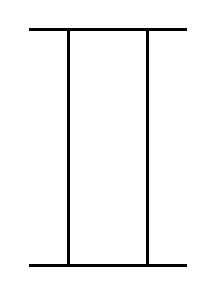
\begin{tikzpicture}[
    % Aumenta a espessura para dar aparência estrutural
    very thick
]

    % ==========================================
    % 1. PRIMEIRO PERFIL (Esquerda)
    % ==========================================
    \draw (-0.5, 0) -- (0.5, 0); % Linha da mesa inferior
    \draw (0, 0) -- (0, 3);  % Linha da alma central
    \draw (-0.5, 3) -- (0.5, 3); % Linha da mesa superior

    % ==========================================
    % 2. SEGUNDO PERFIL (Direita)
    % ==========================================
    % O braço direito do primeiro perfil termina em x=1. 
    % Ao deslocar o eixo do segundo perfil para x=2, os braços se colam.
    \begin{scope}[xshift=1cm]
        \draw (-0.5, 0) -- (0.5, 0); % Linha da mesa inferior
        \draw (0, 0) -- (0, 3);  % Linha da alma central
        \draw (-0.5, 3) -- (0.5, 3); % Linha da mesa superior
    \end{scope}

\end{tikzpicture}

\end{enumerate}